\section{Induction and Recursion}
\subsection{Sequences}
A \textbf{sequence} is a special type of function in which the domain
is the set of consecutive integers.

When a function is specified as a sequence, using subscripts to denote input
is more common, so $g_k$ is used instead of $g(k)$

A value $g_k$ is called a \textbf{term}, and $k$ is the \textit{index} of $g_k$

For example:
\begin{align*}
  g_1 & = 3.67 & g_2 & = 2.88 \\
  g_3 & = 3.25 & g_4 & = 3.75
\end{align*}
\[
  g(k) = 3.67, 2.88, 3.25, 3.75
\]

An entire sequence is denoted by $\{gk\}$, whereas $g_k$ is used to denote a
single term in the sequence.

A sequence commonly starts with $0$ or $1$, but it could be \textit{any} integer.
\subsubsection*{Finite sequence}
A sequence with a finite domain is a \textbf{finite sequence}.
In a finite sequence, there is an \textit{initial index $m$} and a \textit{final index $n$}.
\subsubsection*{Infinite sequence}
A sequence with an infinite domain is a \textbf{infinite sequence}.
In an infinite sequence, there is an \textit{initial index m} and the sequence
is defined for indices $k \geq m$:
\[
  a_m, a_{m+1}, a_{m+2}, a_{m+3}, \ldots
\]
A sequence can be specified by an \textbf{explicit formula}, such as $d_k = 2^k$
for $k \geq 1$.
\[
  \{d_k\} = 2,4,8,16, \ldots
\]
\subsubsection*{Increasing and Decreasing Sequences}
\begin{itemize}
  \item a sequence is \textit{increasing} if for every two consecutive indices, $k$
        and $k+1$, $a_k < a_{k+1}$
  \item a sequence is \textit{non-decreasing} if for every two consecutive indices, $k$
        and $k+1$, $a_k \leq a_{k+1}$
\end{itemize}
For example,
\begin{align*}
  2 < 4 < 5 < 6          & ~\text{increasing \textit{and} non-decreasing}     \\
  2 \leq 4 \leq 5 \leq 6 & ~\text{non-decreasing \textit{but} not increasing}
\end{align*}
\textit{The same relationship can be said for \textbf{decreasing} and \textbf{non-increasing}}.
\subsubsection*{Geometric Sequences}
A \textbf{geometric sequence} is a sequence of real numbers where each term is found by taking
the previous term and multiplying it by a fixed number called the \textbf{common ratio}.

For example, with an \textit{initial term}: 4, and \textit{common ratio}: $\frac{1}{2}$,
\[
  4,2,\frac{1}{2},\frac{1}{4}, \ldots
\]
\subsubsection*{Arithmetic Sequence}
An \textbf{arithmetic sequence} is a sequence of real numbers where each term after the initial
term is found by taking the previous term and adding a fixed number called the \textbf{common difference}.

For example, with an \textit{initial value}: 2, and \textit{common difference}: 3,
\[
  2,5,8,11, \ldots
\]

\subsection{Recurrence relations}
A rule that defines a term $a_n$ as a function of previous terms in the sequence is called a
\textbf{recurrence relation}

For example,
\begin{align*}
  a_0 & = a~\text{initial value} \\
  a_n & = d + a_{n-1}
\end{align*}
Fibonacci Sequence:
\begin{align*}
  f_0 & = 0                                     \\
  f_1 & = 1                                     \\
  f_n & = f_{n-1} + f_{n-2}~\text{for}~n \geq 2 \\
\end{align*}
A \textbf{dynamical system} is a system that changes over time. The state of the system
at any point is determined by a set of well-defined rules that depend on the past states
of the system.

\subsection{Summations}
\textbf{Summation Notation} is used to express the sum of terms in a numerical sequence.
\[
  \sum_{i=s}^{t} a_i = a_{s} + a_{s+1} + \ldots + a_t
\]
\begin{center}
  \begin{tabular}{l}
    $i$ is the \textit{index}       \\
    $s$ is the \textit{lower limit} \\
    $t$ is the \textit{upper limit}
  \end{tabular}
\end{center}
Any variable name could be used for index, but $i,j,k$ and $\ell$
are most common.
\begin{align*}
  \sum_{j=1}^{4} j^3    & :~\text{summation form} \\
  1^3 + 2^3 + 3^3 + 4^3 & :~\text{expanded form}
\end{align*}
\[
  \sum_{k=m}^{n} a_k = \sum_{k=m}^{n-1} a_k + a_n,~\text{for}~n>m
\]
\[
  \sum_{j=1}^{n} (j+2)^3 = \sum_{k=1}^{n} (k+2)^3 = \sum_{i=3}^{n+2} i^3
\]
\subsubsection*{Closed Form}
A \textbf{closed form} for a mathematical sum expresses the value of the sum without
summation notation. For example,
\[
  \sum_{k=0}^{n-1} (a+kd) = an + \frac{d(n-1)n}{2}
\]
\textbf{Arithmetic Sequence Closed Form}:
\[
  \sum_{k=0}^{n-1} (a+kd) = an + \frac{d(n-1)n}{2}
\]
\textbf{Geometric Sequence Closed Form}:
\[
  \sum_{k=0}^{n-1} (a \cdot r^k) = \frac{a(r^n-1)}{r-1}
\]

\subsection{Mathematical induction}
Two Components of an inductive proof:
\begin{itemize}
  \item Base Case:
        \subitem establishes that the theorem is true for the first value in the sequence
  \item Inductive Step:
        \subitem establishes that if the theorem is true for $k$, then the theorem holds for $k+1$
\end{itemize}
\[
  \text{For a}~k \in \mathbb{Z}^+,~s(k) \implies s(k+1)
  \iff [s(1) \implies s(2) \implies s(3) \implies s(4) \implies \cdots]
\]
The supposition that $s(k)$ is true is called the \underline{inductive hypothesis}.

\subsection{More inductive proofs}
Explicit formula for a sequence defined by a recurrence relation
\begin{align*}
  \{g_n\}:~g_0 & =1,~g_n=3g_{n-1} + 2n~\text{then for any $n \geq 0$,} \\
  g_n          & = \frac{5}{2} \cdot 3^n - n - \frac{3}{2}
\end{align*}
\begin{proof}
  by induction on $n$. \\
  Base Case: $n=0$
  \begin{align*}
    g_o & = \frac{5}{2} \cdot 3^0 - 0 - \frac{3}{2} = 1    \\
    g_0 & = 1~\checkmark\quad\text{(by initial condition)}
  \end{align*}
  Inductive Step: assume for any integer $k\geq0$, assume that $g_k=\frac{5}{2} \cdot 3^k-k-\frac{3}{2}$ is true.\\
  For $k+1$:
  \begin{align*}
    g_{k+1} & = 3g_{k} + 2(k+1)\quad\text{by definition}                                  \\
            & = 3(\frac{5}{2}3^k-k-\frac{3}{2})+2(k+1)\quad\text{by induction hypothesis} \\
            & = \frac{5}{2}3^{k+1}-3k-\frac{9}{2}+2k+2                                    \\
            & = \frac{5}{2}3^{k+1}-k-\frac{5}{2}                                          \\
            & = \frac{5}{2}3^{k+1}-(k+1)-\frac{5}{2}\quad\text{by algebra}
  \end{align*}
  $\therefore g_n = \frac{5}{2} \cdot 3^n - n - \frac{3}{2}$, for all $n \in \mathbb{Z}^\geq$
\end{proof}

\subsection{Strong induction and well-ordering}
The \textbf{principle of strong induction} assumes the fact to be proven holds for all values
less than or equal to $k$ and proves the fact holds for $k+1$
\begin{center}
  \begin{tabular}{cllll}
    \multicolumn{5}{c}{Inductive Step for Weak Induction}                  \\
    \hline
    \multicolumn{5}{c}{For all $k\geq1,~S(k) \implies S(k+1)$}             \\
    $k=1$    & $S(1)\implies$ & $S(2)$         &                &          \\
    $k=2$    &                & $S(2)\implies$ & $S(3)$         &          \\
    $k=3$    &                &                & $S(3)\implies$ & $S(4)$   \\
    $\vdots$ &                &                &                & $\ddots$
  \end{tabular}
  \qquad
  \begin{tabular}{cllll}
    \multicolumn{5}{c}{Inductive Step for Strong Induction}                                       \\
    \hline
    \multicolumn{5}{c}{For all $k\geq1,~S(0) \land S(1) \land \ldots \land S(k) \implies S(k+1)$} \\
    $k=1$    & $S(1)\implies$    & $S(2)$            &                &                           \\
    $k=2$    & $S(1)\quad\land $ & $S(2)\implies$    & $S(3)$         &                           \\
    $k=3$    & $S(1)\quad\land $ & $S(2)\quad\land $ & $S(3)\implies$ & $S(4)$                    \\
    $\vdots$ &                   &                   &                & $\ddots$
  \end{tabular}
\end{center}
for $n\geq0,~f_n \leq 2^n$
\begin{proof}
  By Strong Induction of $n$

  Base Case:
  \begin{align*}
    n & = 0:~f_0 = 0 \leq 2^0~\checkmark \\
    n & = 1:~f_1 = 1 \leq 2^1~\checkmark \\
  \end{align*}
  Inductive Step:

  For $k\geq1$, suppose that for any $j$ in the range from $0$ through $k$, $f_k\leq2^j$.
  We will prove that $f_{k+1}\leq2^{k+1}$.

  Since $k\geq1$, then $k-1\geq0$. Therefore both $k$ and $k-1$ fall in the range from
  $0$ through $k$, and by the induction hypothesis $f_{k-1}\leq2^{k-1}$ and $f_k\leq2^k$
  \begin{align*}
    f_{k+1} & = f_k + f_{k-1}              &  & \text{by definition}           \\
            & \leq 2^k + 2^{k-1}           &  & \text{by inductive hypothesis} \\
            & \leq 2^k + 2^{k-1} + 2^{k-1} &  & \text{since $2^{k-1} \geq 0$}  \\
            & \leq 2^k + 2 \cdot 2^{k-1}                                       \\
            & \leq 2^k + 2^k                                                   \\
            & \leq 2 \cdot 2^k                                                 \\
    f_{k+1} & \leq 2^{k+1}                 &  & \text{by algebra}
  \end{align*}
  $\therefore f_{k+1} \leq 2^{k+1}$
\end{proof}

\subsection{Loop invariants}
\subsubsection*{Program Verification}
\begin{itemize}
  \item formally proving that programs perform correctly
  \item behavior is correct if:
        \subitem a pre-condition is true before the program starts
        \subitem a post-condition is true before the program ends
\end{itemize}
\subsubsection*{Loop Invariants for While Loops}
A loop invariant is an assertion that is true before each iteration of a loop.

\subsection{Recursive definitions}
In a recursive definition of a function, the value of the function is defined in term
of the output of the function on smaller input values.

For examples, the factorial:
\begin{align*}
  n!   & = f(n)\quad\text{such that}   \\
  f(0) & = 1                           \\
  f(1) & = n \cdot f(n-1) for n \geq 1
\end{align*}

\subsection{Structural induction}
\textbf{Structural induction} is a type of induction used to prove theorem about recursively
defined sets that follow the structure of the recursive definition.

For example, balanced parenthesis
\begin{align*}
  \text{right}[~))()~]  & = 3 & \text{left}[~)))~] = 0 \\
  \text{left}[~((()))~] & = 3
\end{align*}
Recursive definition for the set of properly nested parenthesis:
\begin{center}
  \begin{tabular}{r|c}
    Basis           & $()\in P$           \\
    Recursive Rules & If $u,v\in P$, then \\
    1               & $(u) \in P$         \\
    2               & $uv \in P$
  \end{tabular}
\end{center}
\textit{Theorem}: If string $x\in P$, then left$[~x~] =$ right $[~x~]$
\begin{proof}
  by structural induction

  \textbf{Base Case}: $() \in P$
  \[
    \text{left}[~()~] = \text{right}[~()~] = 1
  \]

  \textbf{Inductive Step}: If $x\in P$, then $x$ was constructed by apply a sequence
  of recursive rules starting with the string $()$ given in the basis.

  We consider two case, depending on the last recursive rule that was applies to construct $x$.

  \textbf{Case 1} Rules 1 was the last applied to construct $x$.
  Then $x = (u)$, where $u\in P$. We assume that left$[~u~] =$ right $[~u~]$.
  \begin{align*}
    \text{left}[~x~] & = \text{left}[~(u)~]    &  & \text{because $x = (u)$}               \\
                     & = 1 + \text{left}[~u~]  &  & \text{$(u)$ has one more $($ than $u$} \\
                     & = 1 + \text{right}[~u~] &  & \text{by the inductive hypothesis}     \\
                     & = \text{right}[~(u)~]   &  & \text{$(u)$ has one more $)$ than $u$} \\
                     & = \text{right}[~x~]     &  & \text{because $x = (u)$}
  \end{align*}

  \textbf{Case 2} Rule 2 was the last rule applied to construct $x$.
  Then $x=uv$, where $u,v\in P$. We assume that left$[~u~] =$ right $[~u~]$ and left$[~v~] =$ right $[~v~]$.
  \begin{align*}
    \text{left}[~x~] & = \text{left}[~uv~]                     &  & \text{because $x=uv$}          \\
                     & = \text{left}[~u~] + \text{left}[~v~]                                       \\
                     & = \text{right}[~u~] + \text{right}[~v~] &  & \text{by inductive hypothesis} \\
                     & = \text{right}[~uv~]                                                        \\
                     & = \text{right}[~x~]                     &  & \text{because $x=uv$}
  \end{align*}
  $\therefore \text{left}[~x~] = \text{right}[~x~]$
\end{proof}

\subsection{Recursive algorithms}
A \textbf{recursive algorithm} is an algorithm that calls itself.

Ex. a recursive algorithm to compute the factorial formula:
\begin{lstlisting}
  Factorial(n)

  Input:  A non-negative integer n
  Output: n!

  If(n=0), Return(1)
  r := Factorial(n-1) //the recursive call

  Return(r*n)
\end{lstlisting}

Ex. recursive algorithm to compute the powerset of a set:
\begin{lstlisting}
  PowerSet(A)

  Input:  set A
  Output: the powerset of A

  If(A=[emptyset]), return {[emptyset]}

  Select an element a in A
  A' := A - {a}
  P := PowerSet(A') //recursive call
  P' := P
  For each S in P'
    Add (S union {a}) to P
  End-for

  Return(P)
\end{lstlisting}


\subsection{Induction and recursive algorithms}
Nothing very useful in this section, only kept for counting reasons.

\subsection{Analyzing the time complexity of recursive algorithms}
The \textbf{time complexity} of an algorithm is a function $T(n)$, whose $n$ is the input size

Ex. Determining recurrence relation for factorial(n)
\begin{lstlisting}
  Factorial(n)

  If(n=0), Return(1)    // two operations, comparison and returning

  r := Factorial(n-1)   // n-1 recursive calls, 1 operation for assignment

  Return(r*n)           // 2 ops, multiplying and returning
\end{lstlisting}
Therefore, $T(0) = 2$, $T(n) = T(n-1) + 5$

\subsection{Divide-and-conquer algorithms: Introduction and mergesort}
A \textbf{divide-and-conquer} algorithm solves a problem by recursively breaking
the original input into smaller sub-problems of roughly equal size

Ex.
\begin{lstlisting}
  Findmin(L)

  If L has only one item x, return(x)

  Break list L into two lists, A and B

  a := Findmin(A)
  b := Findmin(B)

  If(a <= b) Return(a)
  Else Return(B)
\end{lstlisting}

\subsubsection*{Queue}
A \textbf{queue} maintains items in an ordered list
\begin{itemize}
  \item new items are added to back of queue
  \item items are removed according to first-in, first-out
\end{itemize}
\begin{center}
  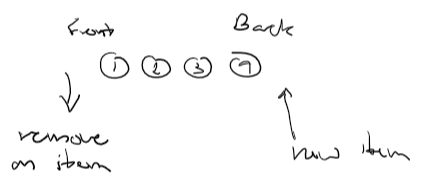
\includegraphics[width=.6\linewidth]{resources/queue.png}
\end{center}

\subsection{Divide-and-conquer algorithms: Binary Search}
\begin{itemize}
  \item A \bld{search algorithm} finds a target in a list.
  \item \bld{Binary Search} is an efficient algorithm to search for a target item in a \itl{sorted list}.
\end{itemize}
{\large Pseudo-code for recursive binary search:}
\begin{lstlisting}
RecBinSearch(low, high, A, x)

If(low = high AND a[low] = x), Return(low)
If(low = high AND a[low] != x), Return(-1)

mid := floor((low + high)/2)

If(x <= a[mid]), then high := mid
If(x > a[mid]), then low := mid+1

Return(RecBinSearch(low, high, A, x))
\end{lstlisting}

\subsection{Solving linear homogeneous recurrence relations}
Finding an explicit formula for a recursively defined sequence is called \itl{solving a recurrence relation}.
\subsubsection*{Linear Homogeneous Recurrence Relation}
A linear homogeneous recurrence relation of degree $k$ has the following form:
\[
  f_n = c_1f_{n-1} + c_2f_{n-2} + \cdots + c_kf_{n-k},
\]
where the $c_j$'s are constants that do not depend on $n$, and $c_k \neq 0$.
\begin{center}
  \begin{tabular}{ll}
    \multicolumn{2}{c}{Examples illustrating linear and non-linear recurrence relations} \\
    \hline
    $b_n = b_{n-1} + (b_{n-2} \cdot b_{n-3})$   & Non-linear                             \\
    $c_n = 3n \cdot c_{n-1}$                    & Non-linear                             \\
    $d_n = d_{n-1} + (d_{n-2})^2$               & Non-linear                             \\
    $f_n = 3f_{n-1} - 2f_{n-2} + f_{n-4} + n^2$ & Linear, degree 4. Non-homogeneous      \\
    $g_n = g_{n-1} + g_{n-3} + 1$               & Linear, degree 3. Non-homogeneous      \\
    $h_n = 2h_{n-1} - h_{n-2}$                  & Linear, degree 2. Homogeneous          \\
    $s_n = 2s_{n-1} = \sqrt{3}s_{n-5}$          & Linear, degree 5. Homogeneous
  \end{tabular}
\end{center}
The expression denoting the infinite set of solutions to a recurrence relation without initial values is called the \itl{general solution} to the recurrence relation.

\subsubsection*{Solutions to linear homogeneous recurrence relations}
If $g_n \tand h_n$ satisfy a linear homogeneous relation then so does $f_n = s\cdot g_n + t\cdot h_n$ for any real numbers $s \tand t$.

\subsubsection*{Using Initial Values to determine to unique solution to a recurrence relation}
Any ${\displaystyle f_n = c_1\left(\frac{1 + \sqrt{5}}{2}\right)^n + c_2\left(\frac{1 - \sqrt{5}}{2}\right)^n}$

\noindent Initial Values:
\begin{align*}
  n & = 0 & f_0 & = 0 = c_1\left(\frac{1 + \sqrt{5}}{2}\right)^0 + c_2\left(\frac{1 - \sqrt{5}}{2}\right)^0 = c_1 + c_2 = 0 \\
  n & = 1 & f_1 & = 1 = c_1\left(\frac{1 + \sqrt{5}}{2}\right) + c_2\left(\frac{1 - \sqrt{5}}{2}\right) = 1
\end{align*}
Then solving a two variable linear system of equations:
\[
  c_1 = \frac{1}{\sqrt{5}}, \qquad c_2 = -\frac{1}{\sqrt{5}}
\]
which then yields the specific solution of
\[
  f_n = \frac{1}{\sqrt{5}}\left(\frac{1 + \sqrt{5}}{2}\right)^n - \frac{1}{\sqrt{5}}\left(\frac{1 - \sqrt{5}}{2}\right)^n.
\]

\subsubsection*{General Steps}
\begin{enumerate}
  \item Use the recurrence relation to find the characteristic equation which will be $p(x) = 0$, where $p(x)$ is a degree $d$ polynomial.
  \item Find all solutions to the characteristic equation. Assume $p(x)$ has distinct roots $x_1, x_2, \ldots, x_d$.
  \item Every solution $f_n = (x_1)^n$ satisfies the recurrence relation. Therefore, any solution of the form $f_n = a_1(x_1)^n + \cdots + a_d(x_d)^n$ satisfies the recurrence relation.
  \item Each initial value gives a value of $f_n$ for a specific value for $n$. Plug the value for $n$ and $f_n$ into the above expression to get a linear equation with variables $a_1,a_2,\ldots,a_d$. There are $d$ linear equations (from the $d$ initial values) and $d$ variables.
  \item Solve for $a_1,a_2,\ldots,a_d$.
  \item Plug values for $a_1,a_2,\ldots,a_d$ back in to the expression for $f_n$ to get the closed form expression for $f_n$.
\end{enumerate}

\subsection{Solving linear non-homogeneous recurrence relations}
A \bld{non-homogeneous linear recurrence relation} is a linear recurrence relation with additional terms that are either a constant or a function of $n$. The recurrence relations below are all examples of homogeneous linear recurrence relations.
\begin{align*}
  f_n & = 3f_{n-1} + 10f_{n-2} + 2   \\
  f_n & = 3f_{n-1} + 10f_{n-2} + 24n \\
  f_n & = 3f_{n-1} + 10f_{n-2} + 3n
\end{align*}
The \bld{associated homogeneous recurrence relation} is the recurrence relation with the additional non-homogeneous terms dropped. For example the associated homogeneous recurrence relation for all of the recurrence relations give above is $f_n = 3f_{n-1} + 10f_{n-2}$.

\subsubsection*{Particular and homogeneous solutions}
The solution to a non-homogeneous linear recurrence relation is the sum of two parts: a \itl{homogeneous solution} plus a \itl{particular solution}. If the sequence is $\{f_n\}$, then the homogeneous solution is denoted by $f_n^{(h)}$ and the particular solution is denoted by $f_n^{(p)}$.
\begin{itemize}
  \item The homogeneous solution $f_n^{(h)}$ is the general solution to the associated homogeneous recurrence relation.
  \item The method for finding the particular solution $f_n^{(p)}$ is to guess the form of the particular solution and then check the guess.
\end{itemize}

\subsubsection*{Summary of all the steps}
\begin{enumerate}
  \item Find the homogeneous part of the solution which is the general solution to the associated homogeneous recurrence relation.
  \item Guess the correct form for the particular solution.
  \item Verify the guess by solving for constants so that the guess satisfies the recurrence relation for all $n$.
  \item Add the homogeneous and particular solutions to get the general solution.
  \item For a degree $d$ linear recurrence relation, there must be $d$ initial values to specify the sequence. Each initial value gives a value for $f_n$ for a specific value for $n$. Plug the values for $n$ and $f_n$ into the general solution to get a linear equation with variables $a_1,a_2,\ldots,a_d$. There are $d$ linear equations (from the $d$ initial values) and $d$ variables.
  \item Solve for $a_1,a_2,\ldots,a_d$.
  \item Plug values for $a_1,a_2,\ldots,a_d$ back in to the general solution for $f_n$ to get the final closed form expression for $f_n$.
\end{enumerate}

\subsection{Divide-and-conquer recurrence relations}
\subsubsection*{Deriving solutions to divide-and-conquer recurrence relations}
Many recurrence relations that describe the time complexity of divide-and-conquer algorithms have the form
\[
  T(n) = aT(n/b) + \Theta(n^d).
\]

\subsubsection*{Expressing the formula as a geometric sum}
The explicit formula for $T(n)$ can be generalized for a recurrence relation of the form $T(n) = aT(n/b) + n^d$ which has an explicit formula
\[
  T(n) = n^d \cdot \sum_{j=0}^{L}\left(\frac{a}{b^d}\right)^j~~\twhere L = \log_b n
\]
The expression for $n^d$ times the sum of terms in a geometric sequence of the form $1 + r + r^2 + \cdots + r^L$, where the ratio $r = a/b^d$. The formula for the sum of a geometric sequence is
\[
  1 + r + r^2 + \cdots + r^L = \sum_{j=0}^{L} r^j = \frac{r^{L+1}-1}{r-1}
\]
The asymptotic growth rate of $T(n)$ depends on whether the ratio $r$ is less than, greater than, or equal to 1.

\subsubsection*{The Master Theorem}
if $T(n) = aT(n/b) + \Theta(n^d)$ for constants $a>0,~b>1,\tand d \geq 0$, then
\begin{itemize}
  \item If $(a/b^d) < 1$, then $T(n) = \Theta(n^d)$
  \item If $(a/b^d) = 1$, then $T(n) = \Theta(n^d \log n)$
  \item If $(a/b^d) > 1$, then $T(n) = \Theta(n^{\log_b a})$
\end{itemize}